\documentclass[11pt,a4paper]{report}

\usepackage[utf8]{inputenc}
\usepackage[T1]{fontenc}\usepackage[spanish]{babel}
\usepackage[notes,backend=biber]{biblatex-chicago}

\usepackage{graphicx}
\usepackage{listings}
\usepackage{float}
\usepackage{csquotes}


\lstset{
	  frame=tb,
	  language=Java,
	  aboveskip=3mm,
	  belowskip=3mm,
	  showstringspaces=false,
	  columns=flexible,
	  basicstyle={\small\ttfamily},
	  numbers=none,
	  breaklines=false,
	  breakatwhitespace=true,
	  tabsize=1
}

\begin{document}
	\begin{titlepage}
		\centering
		{\scshape\huge\bfseries INSTITUTO POLITÉCNICO NACIONAL \par}
		\vspace{0.7cm}
		{\scshape\LARGE\bfseries Escuela Superior de Computo \par}
		\vspace{0.5cm}
		{\scshape\Large \par}
		\vspace{1.5cm}
		{\Large\bfseries Reporte: \par}
		{\huge\bfseries Automatas \par}
		\vspace{2cm}
		{\LARGE\itshape Teoría Computacional\par}
		\vspace{0.2cm}
		{\Large Luis Diego Jimenez Delgado\par}
		\vfill
			{\scshape\Large 2CM5 \par}
			\vspace{0.5cm}
			{\scshape\large Profesor: \par}
			{\scshape\Large Genaro Juarez Martinez \par}
		\vfill
		{\large \today}
	\end{titlepage}
 
	\tableofcontents{}

	\chapter{Autómata de cadena con terminación 01}

	 \section{Diagrama}
		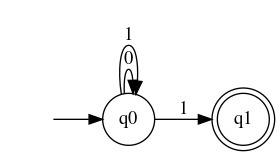
\includegraphics[scale=.80]{D1}

	\section{Código}
			\begin{lstlisting}
				#include <stdlib.h>
				#include "TADColaDin.h"
				#include <stdio.h>

				char getChar();
				void isValidProcess(char initialChar);
				void destroyProcess(cola *porHacer, cola *listos);
				elemento createElemento(int state);
				int manageProcess(cola *porHacer, elemento e, char toEval);
				void moveToAnswer();
				
				FILE *fp;
				FILE *fhelper;
				FILE *fanswer;
				
				int main(int argc, const char **argv)
				{
				    fp = fopen("./file.txt", "r");
				    fanswer = fopen("./answer.txt", "w");
				    char toWork = (char)fgetc(fp);
				    while (toWork != EOF)
				    {
				        isValidProcess(toWork);
				        toWork = (char)fgetc(fp);
				    }
				    fclose(fp);
				    fclose(fanswer);
				    return 0;
				}
				
				char getChar()
				{
				    return (char)fgetc(fp);
				}

				void isValidProcess(char initialChar)
				{
				    cola listos, porHacer;
				    Initialize(&listos);
				    Initialize(&porHacer);
				    manageProcess(&listos, createElemento(0), initialChar);
				    fhelper = fopen("./helper.txt", "w+");
				    while (!Empty(&listos))
				    {
				        while (!Empty(&listos))
				        {
				            int helper = manageProcess(&porHacer, Dequeue(&listos), initialChar);
				            if (helper == 1)
				            {
				                moveToAnswer();
				                destroyProcess(&porHacer,&listos);
				                return;            
				            }
				            else
				            {
				                if (helper == -1)
				                {
				                    destroyProcess(&porHacer,&listos);
				                    return;               
				                }
				            }
				        }
				        if (toEval == ' ' || toEval == '\n' || toWork == EOF){
				            destroyProcess(&porHacer,&listos);
				            return;
				        }
				        while (!Empty(&porHacer))
				        {
				            Queue(&listos, Dequeue(&porHacer));
				        }
				        fputc(initialChar, fhelper);
				        initialChar = getChar();
				    }
				    destroyProcess(&porHacer,&listos);
				    return;
				}
				
				void moveToAnswer()
				{
				    rewind(fhelper);
				    char toWork = (char)fgetc(fhelper);
				    while (toWork != EOF)
				    {
				        fputc(toWork, fanswer);
				        toWork = (char)fgetc(fhelper);
				    }
				    fputc('\n', fanswer);
				}
				
				void destroyProcess(cola *porHacer, cola *listos){
				    Destroy(porHacer);
				    Destroy(listos);
				    fclose(fhelper);
				    remove("./helper.txt");
				}
				
				elemento createElemento(int state)
				{
				    elemento e;
				    e.state = state;
				    return e;
				}
				
				int manageProcess(cola *porHacer, elemento e, char toEval)
				{
				    if (e.state == 0)
				    {
				        if (toEval == '1' || toEval == '0')
				        {
				            Queue(porHacer, createElemento(0));
				            if(toEval == '0'){
				                Queue(porHacer, createElemento(1));
				            }
				        }
				    }
				    else if(e.state ==1){
				        if (toEval == '1')
				        {
				                        Queue(porHacer, createElemento(2));
				        }
				    }
				    else if (e.state == 2)
				    {
				        if (toEval == ' ' || toEval == '\n'){
				            return 1;
				        }
				    }
				    return 0;
				}
	            \end{lstlisting}
	

	\chapter{Idetificador de palabras reservadas en el lenguaje C}
	 
		\section{Descripción}
		 
		Automata c

		\section{Diagrama}
	
	
		\section{Código}
			\begin{lstlisting}
				#include <stdio.h>
				#include <stdlib.h>
				
				/*
				*/
				
				int manage_();
				int manage_a();
				int manage_b();
				int manage_c();
				int manage_d();
				int manage_e();
				int manage_f();
				int manage_g();
				int manage_i();
				int manage_l();
				int manage_r();
				int manage_s();
				int manage_t();
				int manage_u();
				int manage_v();
				int manage_w();
				int manage_au();
				int manage_br();
				int manage_ca();
				int manage_ch();
				int manage_co();
				int manage_de();
				int manage_el();
				int manage_en();
				int manage_ex();
				int manage_fl();
				int manage_fo();
				int manage_go();
				int manage_in();
				int manage_lo();
				int manage_re();
				int manage_sh();
				int manage_si();
				int manage_st();
				int manage_ty();
				int manage_un();
				int manage_vo();
				int manage_wh();
				int manage_aut();
				int manage_bre();
				int manage_cas();
				int manage_cha();
				int manage_con();
				int manage_def();
				int manage_dou();
				int manage_els();
				int manage_enu();
				int manage_ext();
				int manage_flo();
				int manage_got();
				int manage_inc();
				int manage_lon();
				int manage_reg();
				int manage_ret();
				int manage_sho();
				int manage_sig();
				int manage_siz();
				int manage_sta();
				int manage_str();
				int manage_typ();
				int manage_uni();
				int manage_uns();
				int manage_voi();
				int manage_vol();
				int manage_whi();
				int manage_brea();
				int manage_cons();
				int manage_cont();
				int manage_defa();
				int manage_doub();
				int manage_exte();
				int manage_floa();
				int manage_regi();
				int manage_retu();
				int manage_shor();
				int manage_sign();
				int manage_size();
				int manage_stat();
				int manage_stru();
				int manage_type();
				int manage_unio();
				int manage_unsi();
				int manage_vola();
				int manage_whil();
				int manage_incl();
				int manage_conti();
				int manage_defau();
				int manage_doubl();
				int manage_exter();
				int manage_regis();
				int manage_retur();
				int manage_signe();
				int manage_sizeo();
				int manage_stati();
				int manage_struc();
				int manage_typed();
				int manage_unsig();
				int manage_volat();
				int manage_inclu();
				int manage_contin();
				int manage_defaul();
				int manage_regist();
				int manage_typede();
				int manage_unsign();
				int manage_volati();
				int manage_includ();
				int manage_continu();
				int manage_registe();
				int manage_unsigne();
				int manage_volatil();
				
				int lines = 0;
				int char_count = 0;
				
				FILE *file;
				FILE *output;
				
				int main(int argc, const char **argv)
				{
				    int res = 0;
				    file = fopen("./app.c", "r");
				    output = fopen("./answer.txt", "w");
				    while(res != -1)
				    {
				        res = manage_();
				    }
				    fclose(file);
				    fclose(output);
				    return 0;
				}
				
				int register_word(char *word)
				{
				    fprintf(output, "word:%s line:%i char:%i \n", word, lines, char_count - (int) (sizeof(word) / 4)) ;
				    return 1;
				}
				
				char get_char()
				{
				    char_count += 1;
				    return  (char)fgetc(file);
				}
				
				int manage_()
				{
				    char c = get_char();
				    if (c == 'a')
				    {
				        return manage_a();
				    }
				    else if (c == 'b')
				    {
				        return manage_b();
				    }
				    else if (c == 'c')
				    {
				        return manage_c();
				    }
				    else if (c == 'd')
				    {
				        return manage_d();
				    }
				    else if (c == 'e')
				    {
				        return manage_e();
				    }
				    else if (c == 'f')
				    {
				        return manage_f();
				    }
				    else if (c == 'g')
				    {
				        return manage_g();
				    }
				    else if (c == 'i')
				    {
				        return manage_i();
				    }
				    else if (c == 'l')
				    {
				        return manage_l();
				    }
				    else if (c == 'r')
				    {
				        return manage_r();
				    }
				    else if (c == 's')
				    {
				        return manage_s();
				    }
				    else if (c == 't')
				    {
				        return manage_t();
				    }
				    else if (c == 'u')
				    {
				        return manage_u();
				    }
				    else if (c == 'v')
				    {
				        return manage_v();
				    }
				    else if (c == 'w')
				    {
				        return manage_w();
				    }
				    else if (c == '\n')
				    {
				        char_count = 0;
				        lines += 1;
				    }
				    else if (c == EOF)
				    {
				        return -1;
				    }
				    return 0;
				}
	            \end{lstlisting}
	
	{\large\itshape Nota: Se omite el procedimiento debido a la extensión del código. De igual manera se adjunta a continuación el generador de este código.\par}

			\begin{lstlisting}
				import os
				from os.path import isfile, join
				def read_file(path):
				    res = ""
				    with open(path) as fp:
				        line = fp.readline()
				        while line:
				            res += line
				            line = fp.readline()
				    return res
				
				def get_selector(item, count):
				    resa  = ""
				    aux = list()
				    for it in dictio:
				        if it.startswith(item):
				            aux.append(it)
				    dic_aux = list()
				    for it in aux:
				        h = it[count-1:count]
				        if h not in dic_aux:
				            dic_aux.append(h)
				    for it in dic_aux:
				        if item+it in dictio:
				            resa += "else if(c == '"+ it + "'){\n return register_word(\""+ item+it +"\");\n}\n"
				        elif it is not "":
				            methods.append(")
				            resa += "else if(c == '"+ it + "'){\n return manage_" + item+ it+ "();\n}\n"
				    resa = resa[4:]
				    if(item is ""):
				        resa += "else if (c == '\n')\n{\nchar_count = 0;\nlines += 1;\n}\nelse if (c == EOF)\n{\nreturn -1;\n}\nreturn 0;"
				    else:
				        resa += "return 0;"
				    return resa
				
				
				def write_file(name, content):
				    if(os.path.isfile(name)):
				        pass
				    f = open(name, "w+")
				    f.write(content)
				    f.close()
				    return
				
				if __name__ == "__main__":
				    file_content = read_file("dic.txt")
				    dictio = file_content.split("\n")
				    r = 16
				    final = ""
				    methods = list()
				    for i in range(16):
				        res = list()
				        for item in dictio:
				            if len(item) > i:
				                h = item[0:i]
				                if h not in res:
				                    res.append(h)
				        result = ""
				        for item in res:
				            result += ("\nint manage_" + item +  "()\n{\n char c = get_char();\n " + get_selector (item, i + 1)+" \n}\n")
				        final += (result)
				    res_aux = ""
				    for item in methods:
				        res_aux += "\n" + "int manage_" + item+ it+ "();"
				    final = res_aux + final
				    write_file("./a.txt", final)
	            \end{lstlisting}



	\chapter{Autómata de movimientos en un tablero de ajedrez (chessboard)}
	 
		\section{Diagrama}
		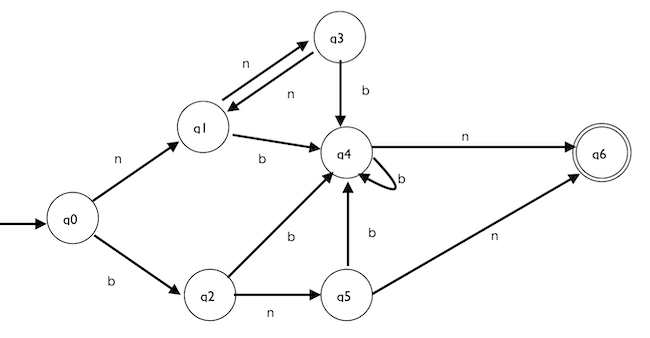
\includegraphics[scale=.80]{diar2}
	
		\section{Código}
			\begin{lstlisting}
#include <stdio.h>
#include <stdlib.h>
#include "TADColaDin.h"

/*

*/

char getChar();
void fillContainer();
void isValidProcess(char initialChar);
void destroyProcess(cola *porHacer, cola *listos);
elemento createElemento(int x, int y);
void manageProcess(cola *porHacer, elemento e, char toEval);
void moveToAnswer(elemento e);
elemento fixElement(elemento toFix);
elemento getEntity(elemento reference, elemento lastFound, char toSearch);
int coordToInt(int x, int y);

void shouldAccept(cola *porHacer, elemento e);

FILE *fp;
FILE *fanswer;
int line = 0;
int turn = 0;

char matrixContainer[3][3];

int main(int argc, const char **argv)
{
    fillContainer();
    fp = fopen("./file.txt", "r");
    fanswer = fopen("./answer.txt", "w");
    char toWork = (char)fgetc(fp);
    while (toWork != EOF)
    {
        isValidProcess(toWork);
        toWork = (char)fgetc(fp);
    }
    fclose(fp);
    fclose(fanswer);
    return 0;
}

void fillContainer()
{
    int i, j, counter = 0;
    for (i = 0; i < 3; ++i)
    {
        for (j = 0; j < 3; ++j)
        {
            if (counter % 2 == 0)
            {
                matrixContainer[i][j] = 'r';
            }
            else
            {
                matrixContainer[i][j] = 'b';
            }
            printf("%c \t", matrixContainer[i][j]);
            ++counter;
        }
        printf("\n");
    }
}

char getChar()
{
    line = 0;
    turn = (turn +1) %2;
    return (char)fgetc(fp);
}

void isValidProcess(char initialChar)
{
    cola listosP1, porHacerP1;
    cola listosP2, porHacerP2;
    Initialize(&listosP1);
    Initialize(&porHacerP1);
    Initialize(&listosP2);
    Initialize(&porHacerP2);
    manageProcess(&listosP1, createElemento(0, 0), initialChar);
    manageProcess(&listosP2, createElemento(2, 2), initialChar);
    while (!Empty(&listosP1)  && !Empty(&listosP2))
    {
        if (initialChar == '\n' || initialChar == ' ' || initialChar == '\0')
        {
            while (!Empty(&listosP1))
            {
              elemento e = Dequeue(&listosP1);
              printf("%i \n", coordToInt(e.x, e.y) );
              if(coordToInt(e.x, e.y) == 9)
              {
                printf("parent = %i line = %i \n", e.line, e.parent);
              } 
            }
            destroyProcess(&porHacerP1, &listosP1);

            while (!Empty(&listosP2))
            {
              elemento e = Dequeue(&listosP2);
              printf("%i \n", coordToInt(e.x, e.y) );
              if(coordToInt(e.x, e.y) == 9)
              {
                printf("parent = %i line = %i \n", e.line, e.parent);
              } 
            }
            destroyProcess(&porHacerP2, &listosP2);
            return;
        }
        while (!Empty(&listosP1))
        {
            manageProcess(&porHacerP1, Dequeue(&listosP1), initialChar);
        }
        while (!Empty(&listosP2))
        {
            manageProcess(&porHacerP2, Dequeue(&listosP2), initialChar);
        }
        while (!Empty(&porHacerP1))
        {
            Queue(&listosP1, Dequeue(&porHacerP1));
        }
        while (!Empty(&porHacerP2))
        {
            Queue(&listosP1, Dequeue(&porHacerP2));
        }
        initialChar = getChar();
    }
    destroyProcess(&porHacerP2, &listosP2);
    destroyProcess(&porHacerP1, &listosP1);
    return;
}

void manageProcess(cola *porHacer, elemento e, char toEval)
{
    elemento aux = e;
    aux.x = aux.x - 1;
    aux.y = aux.y - 1;
    while (aux.x != -3 && aux.y != -3)
    {
        aux = getEntity(e, aux, toEval);
        if(aux.x != -3 && aux.y != -3){
            
            aux.line = line;
            aux.parent = e.line;
            shouldAccept(porHacer, aux);
            ++line;
        }
    }
}

void shouldAccept(cola *porHacer, elemento e)
{
    cola helper;
    boolean valid = TRUE;
    Initialize(&helper);
    while (!Empty(porHacer))
    {
        elemento el =  Dequeue(porHacer);
        
        if (e.x == el.x && e.y == el.y)
        {
            valid = FALSE;
        }

        Queue(&helper, el);
    }
    if(valid)
    {
        Queue(&helper, e);
    }
    while (!Empty(&helper))
    {
        
        elemento el =  Dequeue(&helper);
                Queue(porHacer, el);
    }
    Destroy(&helper);
}

elemento getEntity(elemento reference, elemento lastFound, char toSearch)
{
    elemento e = fixElement(lastFound);
    int startX = e.x;
    int startY = e.y;
    int i, j;
    for (i = startY; i < 3; ++i)
    {
        if (i > reference.y + 1)
            break;
        if (i < reference.y - 1)
            break;
        for (j = startX; j < 3; ++j)
        {
            if (j > reference.x + 1)
                break;
            if (j < reference.x - 1)
                break;
            if (matrixContainer[i][j] == toSearch && ((i != startY) || (j != e.x)))
            {
                return createElemento(j, i);
            }
        }
        startX = 0;
    }
    return createElemento(-3, -3);
}

elemento fixElement(elemento toFix)
{
    elemento e;
    e.x = toFix.x;
    e.y = toFix.y;
    e.line = toFix.line;
    e.parent = toFix.parent;
    if (toFix.x < 0)
        e.x = 0;
    if (toFix.y < 0)
        e.y = 0;
    else
    {
        if (toFix.x > 2)
        {
            e.x = 0;
            e.y = e.y + 1;
        }
    }
    return e;
}

void destroyProcess(cola *porHacer, cola *listos)
{
    Destroy(porHacer);
    Destroy(listos);
}

int coordToInt(int x, int y)
{
    int i, j, counter = 0;
    printf("x = %i y = %i\n", x, y);
    for (i = 0; i < 3; ++i)
    {
        for (j = 0; j < 3; ++j)
        {
            if (i == y && j == x)
            {
                return counter;
            }
            ++ counter;
        }
    }
    return 0;
}

elemento createElemento(int x, int y)
{
    elemento e;
    e.x = x;
    e.y = y;
    e.parent = 0;
    e.line = 0;
    return e;
}

void moveToAnswer(elemento e)
{
    printf("x = %i , y = %i\n", e.x, e.y);
    /*rewind(fhelper);
    char toWork = (char)fgetc(fhelper);
    while (toWork != EOF)
    {
        fputc(toWork, fanswer);
        toWork = (char)fgetc(fhelper);
    }
    fputc('\n', fanswer);*/
}
	            \end{lstlisting}


	\chapter{Generador de expresiones regulares}
	 
	\section{Descripción}
		El siguiente programa genera cadenas aleatorias del Alfabeto definido por el diagrama:
		\section{Diagrama}
		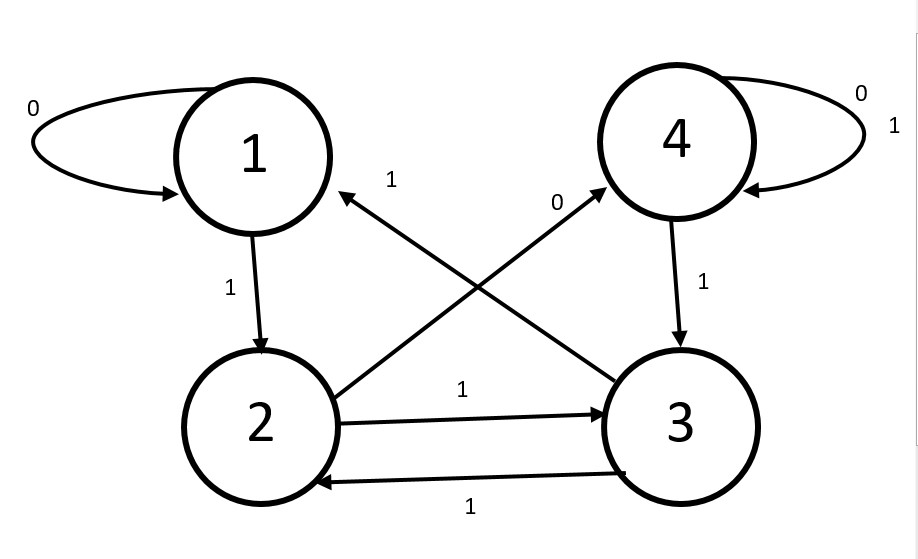
\includegraphics[scale=.50]{D4}

	
		\section{Código}
			\begin{lstlisting}
					#include <stdio.h>
					#include <stdlib.h>
					
					FILE *fanswer;
					
					int getBool();
					void generateString();
					int getRandomNumber(int number);
					
					int main()
					{
					    fanswer = fopen("./answer.txt", "w");
					    int i = 20;
					    while (i != 0)
					    {
					        generateString();
					        --i;
					    }
					    fclose(fanswer);
					}
					
					void generateString()
					{
					    int length = getRandomNumber(100000);
					    while (length >= 0)
					    {
					        if (getBool())
					        {
					            if (getBool())
					            {
					                if (getBool())
					                {
					                    fputc('0', fanswer);
					                }
					                else
					                {
					                    fputc('0', fanswer);
					                    fputc('1', fanswer);
					                    length = length - 1;
					                }
					            }
					            else
					            {
					                fputc('0', fanswer);
					                fputc('1', fanswer);
					                fputc('0', fanswer);
					                length = length - 2;
					            }
					            length = length - 1;
					        }
					        fputc('1', fanswer);
					        length = length - 1;
					    }
					    fputc('\n', fanswer);
					}
					
					int getBool()
					{
					    return getRandomNumber(2);
					}
					
					int getRandomNumber(int number)
					{
					    int res = rand();
					    if (number > 0)
					        res = rand() % number;
					    return res;
					}
	            \end{lstlisting}

\chapter{Ecuaciones}
	 
		
		\section{Diagrama}
		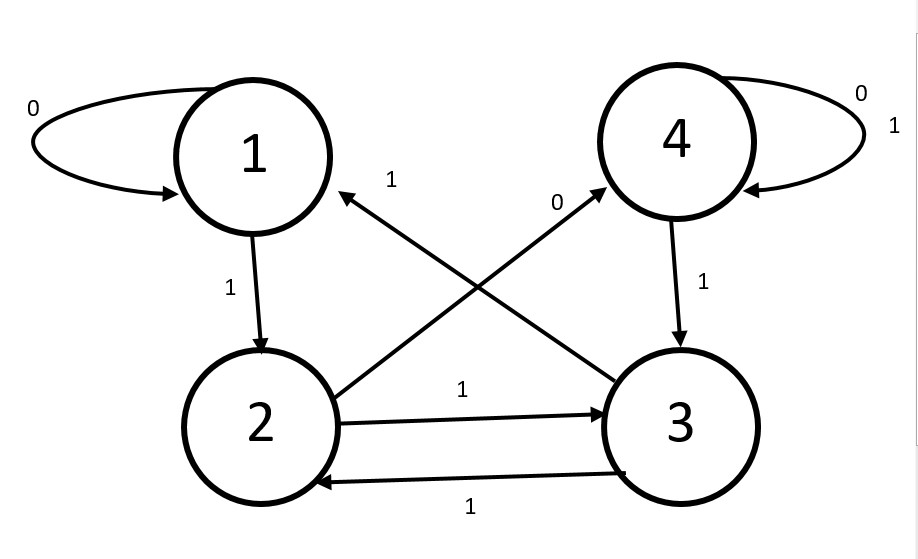
\includegraphics[scale=.50]{D4}

	
		\section{Ecuaciones}
		$R_{11}^{0} = 0$\\
$R_{12}^{0} = 1$\\
$R_{13}^{0} = 11+101$\\
$R_{14}^{0} = 10$\\
$R_{21}^{0} = 11$\\
$R_{22}^{0} = (11)^{*}$\\
$R_{23}^{0} = 1$\\
$R_{24}^{0} = 0$\\
$R_{31}^{0} = 1$\\
$R_{32}^{0} = 1$\\
$R_{33}^{0} = (11)^{*}$\\
$R_{34}^{0} = 110$\\
$R_{41}^{0} = 11$\\
$R_{42}^{0} = 11$\\
$R_{43}^{0} = 1$\\
$R_{44}^{0} = (0)^{*}$\\
$R_{11}^{1} = 0+0(0)^{*}0$\\
$R_{12}^{1} = 1+1(0)^{*}1$\\
$R_{13}^{1} = 11+101+11+101(0)^{*}11+101$\\
$R_{14}^{1} = 10+10(0)^{*}10$\\
$R_{21}^{1} = 11+11(0)^{*}0$\\
$R_{22}^{1} = (11)^{*}+(11)^{*}(0)^{*}1$\\
$R_{23}^{1} = 1+1(0)^{*}11+101$\\
$R_{24}^{1} = 0+0(0)^{*}10$\\
$R_{31}^{1} = 1+1(0)^{*}0$\\
$R_{32}^{1} = 1+1(0)^{*}1$\\
$R_{33}^{1} = (11)^{*}+(11)^{*}(0)^{*}11+101$\\
$R_{34}^{1} = 110+110(0)^{*}10$\\
$R_{41}^{1} = 11+11(0)^{*}0$\\
$R_{42}^{1} = 11+11(0)^{*}1$\\
$R_{43}^{1} = 1+1(0)^{*}11+101$\\
$R_{44}^{1} = (0)^{*}+(0)^{*}(0)^{*}10$\\
$R_{11}^{2} = 0+0(0)^{*}0+0+0(0)^{*}0((11)^{*}+(11)^{*}(0)^{*}1)^{*}11+11(0)^{*}0$\\
$R_{12}^{2} = 1+1(0)^{*}1+1+1(0)^{*}1((11)^{*}+(11)^{*}(0)^{*}1)^{*}(11)^{*}+(11)^{*}(0)^{*}1$\\
$R_{13}^{2} = 11+101+11+101(0)^{*}11+101+11+101+11+101(0)^{*}11+101((11)^{*}+(11)^{*}(0)^{*}1)^{*}1+1(0)^{*}11+101$\\
$R_{14}^{2} = 10+10(0)^{*}10+10+10(0)^{*}10((11)^{*}+(11)^{*}(0)^{*}1)^{*}0+0(0)^{*}10$\\
$R_{21}^{2} = 11+11(0)^{*}0+11+11(0)^{*}0((11)^{*}+(11)^{*}(0)^{*}1)^{*}11+11(0)^{*}0$\\
$R_{22}^{2} = (11)^{*}+(11)^{*}(0)^{*}1+(11)^{*}+(11)^{*}(0)^{*}1((11)^{*}+(11)^{*}(0)^{*}1)^{*}(11)^{*}+(11)^{*}(0)^{*}1$\\
$R_{23}^{2} = 1+1(0)^{*}11+101+1+1(0)^{*}11+101((11)^{*}+(11)^{*}(0)^{*}1)^{*}1+1(0)^{*}11+101$\\
$R_{24}^{2} = 0+0(0)^{*}10+0+0(0)^{*}10((11)^{*}+(11)^{*}(0)^{*}1)^{*}0+0(0)^{*}10$\\
$R_{31}^{2} = 1+1(0)^{*}0+1+1(0)^{*}0((11)^{*}+(11)^{*}(0)^{*}1)^{*}11+11(0)^{*}0$\\
$R_{32}^{2} = 1+1(0)^{*}1+1+1(0)^{*}1((11)^{*}+(11)^{*}(0)^{*}1)^{*}(11)^{*}+(11)^{*}(0)^{*}1$\\
$R_{33}^{2} = (11)^{*}+(11)^{*}(0)^{*}11+101+(11)^{*}+(11)^{*}(0)^{*}11+101((11)^{*}+(11)^{*}(0)^{*}1)^{*}1+1(0)^{*}11+101$\\
$R_{34}^{2} = 110+110(0)^{*}10+110+110(0)^{*}10((11)^{*}+(11)^{*}(0)^{*}1)^{*}0+0(0)^{*}10$\\
$R_{41}^{2} = 11+11(0)^{*}0+11+11(0)^{*}0((11)^{*}+(11)^{*}(0)^{*}1)^{*}11+11(0)^{*}0$\\
$R_{42}^{2} = 11+11(0)^{*}1+11+11(0)^{*}1((11)^{*}+(11)^{*}(0)^{*}1)^{*}(11)^{*}+(11)^{*}(0)^{*}1$\\
$R_{43}^{2} = 1+1(0)^{*}11+101+1+1(0)^{*}11+101((11)^{*}+(11)^{*}(0)^{*}1)^{*}1+1(0)^{*}11+101$\\
$R_{44}^{2} = (0)^{*}+(0)^{*}(0)^{*}10+(0)^{*}+(0)^{*}(0)^{*}10((11)^{*}+(11)^{*}(0)^{*}1)^{*}0+0(0)^{*}10$\\
$R_{11}^{3} = 0+0(0)^{*}0+0+0(0)^{*}0((11)^{*}+(11)^{*}(0)^{*}1)^{*}11+11(0)^{*}0+0+0(0)^{*}0+0+0(0)^{*}0((11)^{*}+(11)^{*}(0)^{*}1)^{*}11+11(0)^{*}0((11)^{*}+(11)^{*}(0)^{*}11+101+(11)^{*}+(11)^{*}(0)^{*}11+101((11)^{*}+(11)^{*}(0)^{*}1)^{*}1+1(0)^{*}11+101)^{*}1+1(0)^{*}0+1+1(0)^{*}0((11)^{*}+(11)^{*}(0)^{*}1)^{*}11+11(0)^{*}0$\\
$R_{12}^{3} = 1+1(0)^{*}1+1+1(0)^{*}1((11)^{*}+(11)^{*}(0)^{*}1)^{*}(11)^{*}+(11)^{*}(0)^{*}1+1+1(0)^{*}1+1+1(0)^{*}1((11)^{*}+(11)^{*}(0)^{*}1)^{*}(11)^{*}+(11)^{*}(0)^{*}1((11)^{*}+(11)^{*}(0)^{*}11+101+(11)^{*}+(11)^{*}(0)^{*}11+101((11)^{*}+(11)^{*}(0)^{*}1)^{*}1+1(0)^{*}11+101)^{*}1+1(0)^{*}1+1+1(0)^{*}1((11)^{*}+(11)^{*}(0)^{*}1)^{*}(11)^{*}+(11)^{*}(0)^{*}1$\\
$R_{13}^{3} = 11+101+11+101(0)^{*}11+101+11+101+11+101(0)^{*}11+101((11)^{*}+(11)^{*}(0)^{*}1)^{*}1+1(0)^{*}11+101+11+101+11+101(0)^{*}11+101+11+101+11+101(0)^{*}11+101((11)^{*}+(11)^{*}(0)^{*}1)^{*}1+1(0)^{*}11+101((11)^{*}+(11)^{*}(0)^{*}11+101+(11)^{*}+(11)^{*}(0)^{*}11+101((11)^{*}+(11)^{*}(0)^{*}1)^{*}1+1(0)^{*}11+101)^{*}(11)^{*}+(11)^{*}(0)^{*}11+101+(11)^{*}+(11)^{*}(0)^{*}11+101((11)^{*}+(11)^{*}(0)^{*}1)^{*}1+1(0)^{*}11+101$\\
$R_{14}^{3} = 10+10(0)^{*}10+10+10(0)^{*}10((11)^{*}+(11)^{*}(0)^{*}1)^{*}0+0(0)^{*}10+10+10(0)^{*}10+10+10(0)^{*}10((11)^{*}+(11)^{*}(0)^{*}1)^{*}0+0(0)^{*}10((11)^{*}+(11)^{*}(0)^{*}11+101+(11)^{*}+(11)^{*}(0)^{*}11+101((11)^{*}+(11)^{*}(0)^{*}1)^{*}1+1(0)^{*}11+101)^{*}110+110(0)^{*}10+110+110(0)^{*}10((11)^{*}+(11)^{*}(0)^{*}1)^{*}0+0(0)^{*}10$\\
$R_{21}^{3} = 11+11(0)^{*}0+11+11(0)^{*}0((11)^{*}+(11)^{*}(0)^{*}1)^{*}11+11(0)^{*}0+11+11(0)^{*}0+11+11(0)^{*}0((11)^{*}+(11)^{*}(0)^{*}1)^{*}11+11(0)^{*}0((11)^{*}+(11)^{*}(0)^{*}11+101+(11)^{*}+(11)^{*}(0)^{*}11+101((11)^{*}+(11)^{*}(0)^{*}1)^{*}1+1(0)^{*}11+101)^{*}1+1(0)^{*}0+1+1(0)^{*}0((11)^{*}+(11)^{*}(0)^{*}1)^{*}11+11(0)^{*}0$\\
$R_{22}^{3} = (11)^{*}+(11)^{*}(0)^{*}1+(11)^{*}+(11)^{*}(0)^{*}1((11)^{*}+(11)^{*}(0)^{*}1)^{*}(11)^{*}+(11)^{*}(0)^{*}1+(11)^{*}+(11)^{*}(0)^{*}1+(11)^{*}+(11)^{*}(0)^{*}1((11)^{*}+(11)^{*}(0)^{*}1)^{*}(11)^{*}+(11)^{*}(0)^{*}1((11)^{*}+(11)^{*}(0)^{*}11+101+(11)^{*}+(11)^{*}(0)^{*}11+101((11)^{*}+(11)^{*}(0)^{*}1)^{*}1+1(0)^{*}11+101)^{*}1+1(0)^{*}1+1+1(0)^{*}1((11)^{*}+(11)^{*}(0)^{*}1)^{*}(11)^{*}+(11)^{*}(0)^{*}1$\\
$R_{23}^{3} = 1+1(0)^{*}11+101+1+1(0)^{*}11+101((11)^{*}+(11)^{*}(0)^{*}1)^{*}1+1(0)^{*}11+101+1+1(0)^{*}11+101+1+1(0)^{*}11+101((11)^{*}+(11)^{*}(0)^{*}1)^{*}1+1(0)^{*}11+101((11)^{*}+(11)^{*}(0)^{*}11+101+(11)^{*}+(11)^{*}(0)^{*}11+101((11)^{*}+(11)^{*}(0)^{*}1)^{*}1+1(0)^{*}11+101)^{*}(11)^{*}+(11)^{*}(0)^{*}11+101+(11)^{*}+(11)^{*}(0)^{*}11+101((11)^{*}+(11)^{*}(0)^{*}1)^{*}1+1(0)^{*}11+101$\\
$R_{24}^{3} = 0+0(0)^{*}10+0+0(0)^{*}10((11)^{*}+(11)^{*}(0)^{*}1)^{*}0+0(0)^{*}10+0+0(0)^{*}10+0+0(0)^{*}10((11)^{*}+(11)^{*}(0)^{*}1)^{*}0+0(0)^{*}10((11)^{*}+(11)^{*}(0)^{*}11+101+(11)^{*}+(11)^{*}(0)^{*}11+101((11)^{*}+(11)^{*}(0)^{*}1)^{*}1+1(0)^{*}11+101)^{*}110+110(0)^{*}10+110+110(0)^{*}10((11)^{*}+(11)^{*}(0)^{*}1)^{*}0+0(0)^{*}10$\\
$R_{31}^{3} = 1+1(0)^{*}0+1+1(0)^{*}0((11)^{*}+(11)^{*}(0)^{*}1)^{*}11+11(0)^{*}0+1+1(0)^{*}0+1+1(0)^{*}0((11)^{*}+(11)^{*}(0)^{*}1)^{*}11+11(0)^{*}0((11)^{*}+(11)^{*}(0)^{*}11+101+(11)^{*}+(11)^{*}(0)^{*}11+101((11)^{*}+(11)^{*}(0)^{*}1)^{*}1+1(0)^{*}11+101)^{*}1+1(0)^{*}0+1+1(0)^{*}0((11)^{*}+(11)^{*}(0)^{*}1)^{*}11+11(0)^{*}0$\\
$R_{32}^{3} = 1+1(0)^{*}1+1+1(0)^{*}1((11)^{*}+(11)^{*}(0)^{*}1)^{*}(11)^{*}+(11)^{*}(0)^{*}1+1+1(0)^{*}1+1+1(0)^{*}1((11)^{*}+(11)^{*}(0)^{*}1)^{*}(11)^{*}+(11)^{*}(0)^{*}1((11)^{*}+(11)^{*}(0)^{*}11+101+(11)^{*}+(11)^{*}(0)^{*}11+101((11)^{*}+(11)^{*}(0)^{*}1)^{*}1+1(0)^{*}11+101)^{*}1+1(0)^{*}1+1+1(0)^{*}1((11)^{*}+(11)^{*}(0)^{*}1)^{*}(11)^{*}+(11)^{*}(0)^{*}1$\\
$R_{33}^{3} = (11)^{*}+(11)^{*}(0)^{*}11+101+(11)^{*}+(11)^{*}(0)^{*}11+101((11)^{*}+(11)^{*}(0)^{*}1)^{*}1+1(0)^{*}11+101+(11)^{*}+(11)^{*}(0)^{*}11+101+(11)^{*}+(11)^{*}(0)^{*}11+101((11)^{*}+(11)^{*}(0)^{*}1)^{*}1+1(0)^{*}11+101((11)^{*}+(11)^{*}(0)^{*}11+101+(11)^{*}+(11)^{*}(0)^{*}11+101((11)^{*}+(11)^{*}(0)^{*}1)^{*}1+1(0)^{*}11+101)^{*}(11)^{*}+(11)^{*}(0)^{*}11+101+(11)^{*}+(11)^{*}(0)^{*}11+101((11)^{*}+(11)^{*}(0)^{*}1)^{*}1+1(0)^{*}11+101$\\
$R_{34}^{3} = 110+110(0)^{*}10+110+110(0)^{*}10((11)^{*}+(11)^{*}(0)^{*}1)^{*}0+0(0)^{*}10+110+110(0)^{*}10+110+110(0)^{*}10((11)^{*}+(11)^{*}(0)^{*}1)^{*}0+0(0)^{*}10((11)^{*}+(11)^{*}(0)^{*}11+101+(11)^{*}+(11)^{*}(0)^{*}11+101((11)^{*}+(11)^{*}(0)^{*}1)^{*}1+1(0)^{*}11+101)^{*}110+110(0)^{*}10+110+110(0)^{*}10((11)^{*}+(11)^{*}(0)^{*}1)^{*}0+0(0)^{*}10$\\
$R_{41}^{3} = 11+11(0)^{*}0+11+11(0)^{*}0((11)^{*}+(11)^{*}(0)^{*}1)^{*}11+11(0)^{*}0+11+11(0)^{*}0+11+11(0)^{*}0((11)^{*}+(11)^{*}(0)^{*}1)^{*}11+11(0)^{*}0((11)^{*}+(11)^{*}(0)^{*}11+101+(11)^{*}+(11)^{*}(0)^{*}11+101((11)^{*}+(11)^{*}(0)^{*}1)^{*}1+1(0)^{*}11+101)^{*}1+1(0)^{*}0+1+1(0)^{*}0((11)^{*}+(11)^{*}(0)^{*}1)^{*}11+11(0)^{*}0$\\
$R_{42}^{3} = 11+11(0)^{*}1+11+11(0)^{*}1((11)^{*}+(11)^{*}(0)^{*}1)^{*}(11)^{*}+(11)^{*}(0)^{*}1+11+11(0)^{*}1+11+11(0)^{*}1((11)^{*}+(11)^{*}(0)^{*}1)^{*}(11)^{*}+(11)^{*}(0)^{*}1((11)^{*}+(11)^{*}(0)^{*}11+101+(11)^{*}+(11)^{*}(0)^{*}11+101((11)^{*}+(11)^{*}(0)^{*}1)^{*}1+1(0)^{*}11+101)^{*}1+1(0)^{*}1+1+1(0)^{*}1((11)^{*}+(11)^{*}(0)^{*}1)^{*}(11)^{*}+(11)^{*}(0)^{*}1$\\
$R_{43}^{3} = 1+1(0)^{*}11+101+1+1(0)^{*}11+101((11)^{*}+(11)^{*}(0)^{*}1)^{*}1+1(0)^{*}11+101+1+1(0)^{*}11+101+1+1(0)^{*}11+101((11)^{*}+(11)^{*}(0)^{*}1)^{*}1+1(0)^{*}11+101((11)^{*}+(11)^{*}(0)^{*}11+101+(11)^{*}+(11)^{*}(0)^{*}11+101((11)^{*}+(11)^{*}(0)^{*}1)^{*}1+1(0)^{*}11+101)^{*}(11)^{*}+(11)^{*}(0)^{*}11+101+(11)^{*}+(11)^{*}(0)^{*}11+101((11)^{*}+(11)^{*}(0)^{*}1)^{*}1+1(0)^{*}11+101$\\
$R_{44}^{3} = (0)^{*}+(0)^{*}(0)^{*}10+(0)^{*}+(0)^{*}(0)^{*}10((11)^{*}+(11)^{*}(0)^{*}1)^{*}0+0(0)^{*}10+(0)^{*}+(0)^{*}(0)^{*}10+(0)^{*}+(0)^{*}(0)^{*}10((11)^{*}+(11)^{*}(0)^{*}1)^{*}0+0(0)^{*}10((11)^{*}+(11)^{*}(0)^{*}11+101+(11)^{*}+(11)^{*}(0)^{*}11+101((11)^{*}+(11)^{*}(0)^{*}1)^{*}1+1(0)^{*}11+101)^{*}110+110(0)^{*}10+110+110(0)^{*}10((11)^{*}+(11)^{*}(0)^{*}1)^{*}0+0(0)^{*}10$\\
$R_{11}^{4} = 0+0(0)^{*}0+0+0(0)^{*}0((11)^{*}+(11)^{*}(0)^{*}1)^{*}11+11(0)^{*}0+0+0(0)^{*}0+0+0(0)^{*}0((11)^{*}+(11)^{*}(0)^{*}1)^{*}11+11(0)^{*}0((11)^{*}+(11)^{*}(0)^{*}11+101+(11)^{*}+(11)^{*}(0)^{*}11+101((11)^{*}+(11)^{*}(0)^{*}1)^{*}1+1(0)^{*}11+101)^{*}1+1(0)^{*}0+1+1(0)^{*}0((11)^{*}+(11)^{*}(0)^{*}1)^{*}11+11(0)^{*}0+0+0(0)^{*}0+0+0(0)^{*}0((11)^{*}+(11)^{*}(0)^{*}1)^{*}11+11(0)^{*}0+0+0(0)^{*}0+0+0(0)^{*}0((11)^{*}+(11)^{*}(0)^{*}1)^{*}11+11(0)^{*}0((11)^{*}+(11)^{*}(0)^{*}11+101+(11)^{*}+(11)^{*}(0)^{*}11+101((11)^{*}+(11)^{*}(0)^{*}1)^{*}1+1(0)^{*}11+101)^{*}1+1(0)^{*}0+1+1(0)^{*}0((11)^{*}+(11)^{*}(0)^{*}1)^{*}11+11(0)^{*}0((0)^{*}+(0)^{*}(0)^{*}10+(0)^{*}+(0)^{*}(0)^{*}10((11)^{*}+(11)^{*}(0)^{*}1)^{*}0+0(0)^{*}10+(0)^{*}+(0)^{*}(0)^{*}10+(0)^{*}+(0)^{*}(0)^{*}10((11)^{*}+(11)^{*}(0)^{*}1)^{*}0+0(0)^{*}10((11)^{*}+(11)^{*}(0)^{*}11+101+(11)^{*}+(11)^{*}(0)^{*}11+101((11)^{*}+(11)^{*}(0)^{*}1)^{*}1+1(0)^{*}11+101)^{*}110+110(0)^{*}10+110+110(0)^{*}10((11)^{*}+(11)^{*}(0)^{*}1)^{*}0+0(0)^{*}10)^{*}11+11(0)^{*}0+11+11(0)^{*}0((11)^{*}+(11)^{*}(0)^{*}1)^{*}11+11(0)^{*}0+11+11(0)^{*}0+11+11(0)^{*}0((11)^{*}+(11)^{*}(0)^{*}1)^{*}11+11(0)^{*}0((11)^{*}+(11)^{*}(0)^{*}11+101+(11)^{*}+(11)^{*}(0)^{*}11+101((11)^{*}+(11)^{*}(0)^{*}1)^{*}1+1(0)^{*}11+101)^{*}1+1(0)^{*}0+1+1(0)^{*}0((11)^{*}+(11)^{*}(0)^{*}1)^{*}11+11(0)^{*}0$\\
$R_{12}^{4} = 1+1(0)^{*}1+1+1(0)^{*}1((11)^{*}+(11)^{*}(0)^{*}1)^{*}(11)^{*}+(11)^{*}(0)^{*}1+1+1(0)^{*}1+1+1(0)^{*}1((11)^{*}+(11)^{*}(0)^{*}1)^{*}(11)^{*}+(11)^{*}(0)^{*}1((11)^{*}+(11)^{*}(0)^{*}11+101+(11)^{*}+(11)^{*}(0)^{*}11+101((11)^{*}+(11)^{*}(0)^{*}1)^{*}1+1(0)^{*}11+101)^{*}1+1(0)^{*}1+1+1(0)^{*}1((11)^{*}+(11)^{*}(0)^{*}1)^{*}(11)^{*}+(11)^{*}(0)^{*}1+1+1(0)^{*}1+1+1(0)^{*}1((11)^{*}+(11)^{*}(0)^{*}1)^{*}(11)^{*}+(11)^{*}(0)^{*}1+1+1(0)^{*}1+1+1(0)^{*}1((11)^{*}+(11)^{*}(0)^{*}1)^{*}(11)^{*}+(11)^{*}(0)^{*}1((11)^{*}+(11)^{*}(0)^{*}11+101+(11)^{*}+(11)^{*}(0)^{*}11+101((11)^{*}+(11)^{*}(0)^{*}1)^{*}1+1(0)^{*}11+101)^{*}1+1(0)^{*}1+1+1(0)^{*}1((11)^{*}+(11)^{*}(0)^{*}1)^{*}(11)^{*}+(11)^{*}(0)^{*}1((0)^{*}+(0)^{*}(0)^{*}10+(0)^{*}+(0)^{*}(0)^{*}10((11)^{*}+(11)^{*}(0)^{*}1)^{*}0+0(0)^{*}10+(0)^{*}+(0)^{*}(0)^{*}10+(0)^{*}+(0)^{*}(0)^{*}10((11)^{*}+(11)^{*}(0)^{*}1)^{*}0+0(0)^{*}10((11)^{*}+(11)^{*}(0)^{*}11+101+(11)^{*}+(11)^{*}(0)^{*}11+101((11)^{*}+(11)^{*}(0)^{*}1)^{*}1+1(0)^{*}11+101)^{*}110+110(0)^{*}10+110+110(0)^{*}10((11)^{*}+(11)^{*}(0)^{*}1)^{*}0+0(0)^{*}10)^{*}11+11(0)^{*}1+11+11(0)^{*}1((11)^{*}+(11)^{*}(0)^{*}1)^{*}(11)^{*}+(11)^{*}(0)^{*}1+11+11(0)^{*}1+11+11(0)^{*}1((11)^{*}+(11)^{*}(0)^{*}1)^{*}(11)^{*}+(11)^{*}(0)^{*}1((11)^{*}+(11)^{*}(0)^{*}11+101+(11)^{*}+(11)^{*}(0)^{*}11+101((11)^{*}+(11)^{*}(0)^{*}1)^{*}1+1(0)^{*}11+101)^{*}1+1(0)^{*}1+1+1(0)^{*}1((11)^{*}+(11)^{*}(0)^{*}1)^{*}(11)^{*}+(11)^{*}(0)^{*}1$\\
$R_{13}^{4} = 11+101+11+101(0)^{*}11+101+11+101+11+101(0)^{*}11+101((11)^{*}+(11)^{*}(0)^{*}1)^{*}1+1(0)^{*}11+101+11+101+11+101(0)^{*}11+101+11+101+11+101(0)^{*}11+101((11)^{*}+(11)^{*}(0)^{*}1)^{*}1+1(0)^{*}11+101((11)^{*}+(11)^{*}(0)^{*}11+101+(11)^{*}+(11)^{*}(0)^{*}11+101((11)^{*}+(11)^{*}(0)^{*}1)^{*}1+1(0)^{*}11+101)^{*}(11)^{*}+(11)^{*}(0)^{*}11+101+(11)^{*}+(11)^{*}(0)^{*}11+101((11)^{*}+(11)^{*}(0)^{*}1)^{*}1+1(0)^{*}11+101+11+101+11+101(0)^{*}11+101+11+101+11+101(0)^{*}11+101((11)^{*}+(11)^{*}(0)^{*}1)^{*}1+1(0)^{*}11+101+11+101+11+101(0)^{*}11+101+11+101+11+101(0)^{*}11+101((11)^{*}+(11)^{*}(0)^{*}1)^{*}1+1(0)^{*}11+101((11)^{*}+(11)^{*}(0)^{*}11+101+(11)^{*}+(11)^{*}(0)^{*}11+101((11)^{*}+(11)^{*}(0)^{*}1)^{*}1+1(0)^{*}11+101)^{*}(11)^{*}+(11)^{*}(0)^{*}11+101+(11)^{*}+(11)^{*}(0)^{*}11+101((11)^{*}+(11)^{*}(0)^{*}1)^{*}1+1(0)^{*}11+101((0)^{*}+(0)^{*}(0)^{*}10+(0)^{*}+(0)^{*}(0)^{*}10((11)^{*}+(11)^{*}(0)^{*}1)^{*}0+0(0)^{*}10+(0)^{*}+(0)^{*}(0)^{*}10+(0)^{*}+(0)^{*}(0)^{*}10((11)^{*}+(11)^{*}(0)^{*}1)^{*}0+0(0)^{*}10((11)^{*}+(11)^{*}(0)^{*}11+101+(11)^{*}+(11)^{*}(0)^{*}11+101((11)^{*}+(11)^{*}(0)^{*}1)^{*}1+1(0)^{*}11+101)^{*}110+110(0)^{*}10+110+110(0)^{*}10((11)^{*}+(11)^{*}(0)^{*}1)^{*}0+0(0)^{*}10)^{*}1+1(0)^{*}11+101+1+1(0)^{*}11+101((11)^{*}+(11)^{*}(0)^{*}1)^{*}1+1(0)^{*}11+101+1+1(0)^{*}11+101+1+1(0)^{*}11+101((11)^{*}+(11)^{*}(0)^{*}1)^{*}1+1(0)^{*}11+101((11)^{*}+(11)^{*}(0)^{*}11+101+(11)^{*}+(11)^{*}(0)^{*}11+101((11)^{*}+(11)^{*}(0)^{*}1)^{*}1+1(0)^{*}11+101)^{*}(11)^{*}+(11)^{*}(0)^{*}11+101+(11)^{*}+(11)^{*}(0)^{*}11+101((11)^{*}+(11)^{*}(0)^{*}1)^{*}1+1(0)^{*}11+101$\\
$R_{14}^{4} = 10+10(0)^{*}10+10+10(0)^{*}10((11)^{*}+(11)^{*}(0)^{*}1)^{*}0+0(0)^{*}10+10+10(0)^{*}10+10+10(0)^{*}10((11)^{*}+(11)^{*}(0)^{*}1)^{*}0+0(0)^{*}10((11)^{*}+(11)^{*}(0)^{*}11+101+(11)^{*}+(11)^{*}(0)^{*}11+101((11)^{*}+(11)^{*}(0)^{*}1)^{*}1+1(0)^{*}11+101)^{*}110+110(0)^{*}10+110+110(0)^{*}10((11)^{*}+(11)^{*}(0)^{*}1)^{*}0+0(0)^{*}10+10+10(0)^{*}10+10+10(0)^{*}10((11)^{*}+(11)^{*}(0)^{*}1)^{*}0+0(0)^{*}10+10+10(0)^{*}10+10+10(0)^{*}10((11)^{*}+(11)^{*}(0)^{*}1)^{*}0+0(0)^{*}10((11)^{*}+(11)^{*}(0)^{*}11+101+(11)^{*}+(11)^{*}(0)^{*}11+101((11)^{*}+(11)^{*}(0)^{*}1)^{*}1+1(0)^{*}11+101)^{*}110+110(0)^{*}10+110+110(0)^{*}10((11)^{*}+(11)^{*}(0)^{*}1)^{*}0+0(0)^{*}10((0)^{*}+(0)^{*}(0)^{*}10+(0)^{*}+(0)^{*}(0)^{*}10((11)^{*}+(11)^{*}(0)^{*}1)^{*}0+0(0)^{*}10+(0)^{*}+(0)^{*}(0)^{*}10+(0)^{*}+(0)^{*}(0)^{*}10((11)^{*}+(11)^{*}(0)^{*}1)^{*}0+0(0)^{*}10((11)^{*}+(11)^{*}(0)^{*}11+101+(11)^{*}+(11)^{*}(0)^{*}11+101((11)^{*}+(11)^{*}(0)^{*}1)^{*}1+1(0)^{*}11+101)^{*}110+110(0)^{*}10+110+110(0)^{*}10((11)^{*}+(11)^{*}(0)^{*}1)^{*}0+0(0)^{*}10)^{*}(0)^{*}+(0)^{*}(0)^{*}10+(0)^{*}+(0)^{*}(0)^{*}10((11)^{*}+(11)^{*}(0)^{*}1)^{*}0+0(0)^{*}10+(0)^{*}+(0)^{*}(0)^{*}10+(0)^{*}+(0)^{*}(0)^{*}10((11)^{*}+(11)^{*}(0)^{*}1)^{*}0+0(0)^{*}10((11)^{*}+(11)^{*}(0)^{*}11+101+(11)^{*}+(11)^{*}(0)^{*}11+101((11)^{*}+(11)^{*}(0)^{*}1)^{*}1+1(0)^{*}11+101)^{*}110+110(0)^{*}10+110+110(0)^{*}10((11)^{*}+(11)^{*}(0)^{*}1)^{*}0+0(0)^{*}10$\\
$R_{21}^{4} = 11+11(0)^{*}0+11+11(0)^{*}0((11)^{*}+(11)^{*}(0)^{*}1)^{*}11+11(0)^{*}0+11+11(0)^{*}0+11+11(0)^{*}0((11)^{*}+(11)^{*}(0)^{*}1)^{*}11+11(0)^{*}0((11)^{*}+(11)^{*}(0)^{*}11+101+(11)^{*}+(11)^{*}(0)^{*}11+101((11)^{*}+(11)^{*}(0)^{*}1)^{*}1+1(0)^{*}11+101)^{*}1+1(0)^{*}0+1+1(0)^{*}0((11)^{*}+(11)^{*}(0)^{*}1)^{*}11+11(0)^{*}0+11+11(0)^{*}0+11+11(0)^{*}0((11)^{*}+(11)^{*}(0)^{*}1)^{*}11+11(0)^{*}0+11+11(0)^{*}0+11+11(0)^{*}0((11)^{*}+(11)^{*}(0)^{*}1)^{*}11+11(0)^{*}0((11)^{*}+(11)^{*}(0)^{*}11+101+(11)^{*}+(11)^{*}(0)^{*}11+101((11)^{*}+(11)^{*}(0)^{*}1)^{*}1+1(0)^{*}11+101)^{*}1+1(0)^{*}0+1+1(0)^{*}0((11)^{*}+(11)^{*}(0)^{*}1)^{*}11+11(0)^{*}0((0)^{*}+(0)^{*}(0)^{*}10+(0)^{*}+(0)^{*}(0)^{*}10((11)^{*}+(11)^{*}(0)^{*}1)^{*}0+0(0)^{*}10+(0)^{*}+(0)^{*}(0)^{*}10+(0)^{*}+(0)^{*}(0)^{*}10((11)^{*}+(11)^{*}(0)^{*}1)^{*}0+0(0)^{*}10((11)^{*}+(11)^{*}(0)^{*}11+101+(11)^{*}+(11)^{*}(0)^{*}11+101((11)^{*}+(11)^{*}(0)^{*}1)^{*}1+1(0)^{*}11+101)^{*}110+110(0)^{*}10+110+110(0)^{*}10((11)^{*}+(11)^{*}(0)^{*}1)^{*}0+0(0)^{*}10)^{*}11+11(0)^{*}0+11+11(0)^{*}0((11)^{*}+(11)^{*}(0)^{*}1)^{*}11+11(0)^{*}0+11+11(0)^{*}0+11+11(0)^{*}0((11)^{*}+(11)^{*}(0)^{*}1)^{*}11+11(0)^{*}0((11)^{*}+(11)^{*}(0)^{*}11+101+(11)^{*}+(11)^{*}(0)^{*}11+101((11)^{*}+(11)^{*}(0)^{*}1)^{*}1+1(0)^{*}11+101)^{*}1+1(0)^{*}0+1+1(0)^{*}0((11)^{*}+(11)^{*}(0)^{*}1)^{*}11+11(0)^{*}0$\\
$R_{22}^{4} = (11)^{*}+(11)^{*}(0)^{*}1+(11)^{*}+(11)^{*}(0)^{*}1((11)^{*}+(11)^{*}(0)^{*}1)^{*}(11)^{*}+(11)^{*}(0)^{*}1+(11)^{*}+(11)^{*}(0)^{*}1+(11)^{*}+(11)^{*}(0)^{*}1((11)^{*}+(11)^{*}(0)^{*}1)^{*}(11)^{*}+(11)^{*}(0)^{*}1((11)^{*}+(11)^{*}(0)^{*}11+101+(11)^{*}+(11)^{*}(0)^{*}11+101((11)^{*}+(11)^{*}(0)^{*}1)^{*}1+1(0)^{*}11+101)^{*}1+1(0)^{*}1+1+1(0)^{*}1((11)^{*}+(11)^{*}(0)^{*}1)^{*}(11)^{*}+(11)^{*}(0)^{*}1+(11)^{*}+(11)^{*}(0)^{*}1+(11)^{*}+(11)^{*}(0)^{*}1((11)^{*}+(11)^{*}(0)^{*}1)^{*}(11)^{*}+(11)^{*}(0)^{*}1+(11)^{*}+(11)^{*}(0)^{*}1+(11)^{*}+(11)^{*}(0)^{*}1((11)^{*}+(11)^{*}(0)^{*}1)^{*}(11)^{*}+(11)^{*}(0)^{*}1((11)^{*}+(11)^{*}(0)^{*}11+101+(11)^{*}+(11)^{*}(0)^{*}11+101((11)^{*}+(11)^{*}(0)^{*}1)^{*}1+1(0)^{*}11+101)^{*}1+1(0)^{*}1+1+1(0)^{*}1((11)^{*}+(11)^{*}(0)^{*}1)^{*}(11)^{*}+(11)^{*}(0)^{*}1((0)^{*}+(0)^{*}(0)^{*}10+(0)^{*}+(0)^{*}(0)^{*}10((11)^{*}+(11)^{*}(0)^{*}1)^{*}0+0(0)^{*}10+(0)^{*}+(0)^{*}(0)^{*}10+(0)^{*}+(0)^{*}(0)^{*}10((11)^{*}+(11)^{*}(0)^{*}1)^{*}0+0(0)^{*}10((11)^{*}+(11)^{*}(0)^{*}11+101+(11)^{*}+(11)^{*}(0)^{*}11+101((11)^{*}+(11)^{*}(0)^{*}1)^{*}1+1(0)^{*}11+101)^{*}110+110(0)^{*}10+110+110(0)^{*}10((11)^{*}+(11)^{*}(0)^{*}1)^{*}0+0(0)^{*}10)^{*}11+11(0)^{*}1+11+11(0)^{*}1((11)^{*}+(11)^{*}(0)^{*}1)^{*}(11)^{*}+(11)^{*}(0)^{*}1+11+11(0)^{*}1+11+11(0)^{*}1((11)^{*}+(11)^{*}(0)^{*}1)^{*}(11)^{*}+(11)^{*}(0)^{*}1((11)^{*}+(11)^{*}(0)^{*}11+101+(11)^{*}+(11)^{*}(0)^{*}11+101((11)^{*}+(11)^{*}(0)^{*}1)^{*}1+1(0)^{*}11+101)^{*}1+1(0)^{*}1+1+1(0)^{*}1((11)^{*}+(11)^{*}(0)^{*}1)^{*}(11)^{*}+(11)^{*}(0)^{*}1$\\
$R_{23}^{4} = 1+1(0)^{*}11+101+1+1(0)^{*}11+101((11)^{*}+(11)^{*}(0)^{*}1)^{*}1+1(0)^{*}11+101+1+1(0)^{*}11+101+1+1(0)^{*}11+101((11)^{*}+(11)^{*}(0)^{*}1)^{*}1+1(0)^{*}11+101((11)^{*}+(11)^{*}(0)^{*}11+101+(11)^{*}+(11)^{*}(0)^{*}11+101((11)^{*}+(11)^{*}(0)^{*}1)^{*}1+1(0)^{*}11+101)^{*}(11)^{*}+(11)^{*}(0)^{*}11+101+(11)^{*}+(11)^{*}(0)^{*}11+101((11)^{*}+(11)^{*}(0)^{*}1)^{*}1+1(0)^{*}11+101+1+1(0)^{*}11+101+1+1(0)^{*}11+101((11)^{*}+(11)^{*}(0)^{*}1)^{*}1+1(0)^{*}11+101+1+1(0)^{*}11+101+1+1(0)^{*}11+101((11)^{*}+(11)^{*}(0)^{*}1)^{*}1+1(0)^{*}11+101((11)^{*}+(11)^{*}(0)^{*}11+101+(11)^{*}+(11)^{*}(0)^{*}11+101((11)^{*}+(11)^{*}(0)^{*}1)^{*}1+1(0)^{*}11+101)^{*}(11)^{*}+(11)^{*}(0)^{*}11+101+(11)^{*}+(11)^{*}(0)^{*}11+101((11)^{*}+(11)^{*}(0)^{*}1)^{*}1+1(0)^{*}11+101((0)^{*}+(0)^{*}(0)^{*}10+(0)^{*}+(0)^{*}(0)^{*}10((11)^{*}+(11)^{*}(0)^{*}1)^{*}0+0(0)^{*}10+(0)^{*}+(0)^{*}(0)^{*}10+(0)^{*}+(0)^{*}(0)^{*}10((11)^{*}+(11)^{*}(0)^{*}1)^{*}0+0(0)^{*}10((11)^{*}+(11)^{*}(0)^{*}11+101+(11)^{*}+(11)^{*}(0)^{*}11+101((11)^{*}+(11)^{*}(0)^{*}1)^{*}1+1(0)^{*}11+101)^{*}110+110(0)^{*}10+110+110(0)^{*}10((11)^{*}+(11)^{*}(0)^{*}1)^{*}0+0(0)^{*}10)^{*}1+1(0)^{*}11+101+1+1(0)^{*}11+101((11)^{*}+(11)^{*}(0)^{*}1)^{*}1+1(0)^{*}11+101+1+1(0)^{*}11+101+1+1(0)^{*}11+101((11)^{*}+(11)^{*}(0)^{*}1)^{*}1+1(0)^{*}11+101((11)^{*}+(11)^{*}(0)^{*}11+101+(11)^{*}+(11)^{*}(0)^{*}11+101((11)^{*}+(11)^{*}(0)^{*}1)^{*}1+1(0)^{*}11+101)^{*}(11)^{*}+(11)^{*}(0)^{*}11+101+(11)^{*}+(11)^{*}(0)^{*}11+101((11)^{*}+(11)^{*}(0)^{*}1)^{*}1+1(0)^{*}11+101$\\
$R_{24}^{4} = 0+0(0)^{*}10+0+0(0)^{*}10((11)^{*}+(11)^{*}(0)^{*}1)^{*}0+0(0)^{*}10+0+0(0)^{*}10+0+0(0)^{*}10((11)^{*}+(11)^{*}(0)^{*}1)^{*}0+0(0)^{*}10((11)^{*}+(11)^{*}(0)^{*}11+101+(11)^{*}+(11)^{*}(0)^{*}11+101((11)^{*}+(11)^{*}(0)^{*}1)^{*}1+1(0)^{*}11+101)^{*}110+110(0)^{*}10+110+110(0)^{*}10((11)^{*}+(11)^{*}(0)^{*}1)^{*}0+0(0)^{*}10+0+0(0)^{*}10+0+0(0)^{*}10((11)^{*}+(11)^{*}(0)^{*}1)^{*}0+0(0)^{*}10+0+0(0)^{*}10+0+0(0)^{*}10((11)^{*}+(11)^{*}(0)^{*}1)^{*}0+0(0)^{*}10((11)^{*}+(11)^{*}(0)^{*}11+101+(11)^{*}+(11)^{*}(0)^{*}11+101((11)^{*}+(11)^{*}(0)^{*}1)^{*}1+1(0)^{*}11+101)^{*}110+110(0)^{*}10+110+110(0)^{*}10((11)^{*}+(11)^{*}(0)^{*}1)^{*}0+0(0)^{*}10((0)^{*}+(0)^{*}(0)^{*}10+(0)^{*}+(0)^{*}(0)^{*}10((11)^{*}+(11)^{*}(0)^{*}1)^{*}0+0(0)^{*}10+(0)^{*}+(0)^{*}(0)^{*}10+(0)^{*}+(0)^{*}(0)^{*}10((11)^{*}+(11)^{*}(0)^{*}1)^{*}0+0(0)^{*}10((11)^{*}+(11)^{*}(0)^{*}11+101+(11)^{*}+(11)^{*}(0)^{*}11+101((11)^{*}+(11)^{*}(0)^{*}1)^{*}1+1(0)^{*}11+101)^{*}110+110(0)^{*}10+110+110(0)^{*}10((11)^{*}+(11)^{*}(0)^{*}1)^{*}0+0(0)^{*}10)^{*}(0)^{*}+(0)^{*}(0)^{*}10+(0)^{*}+(0)^{*}(0)^{*}10((11)^{*}+(11)^{*}(0)^{*}1)^{*}0+0(0)^{*}10+(0)^{*}+(0)^{*}(0)^{*}10+(0)^{*}+(0)^{*}(0)^{*}10((11)^{*}+(11)^{*}(0)^{*}1)^{*}0+0(0)^{*}10((11)^{*}+(11)^{*}(0)^{*}11+101+(11)^{*}+(11)^{*}(0)^{*}11+101((11)^{*}+(11)^{*}(0)^{*}1)^{*}1+1(0)^{*}11+101)^{*}110+110(0)^{*}10+110+110(0)^{*}10((11)^{*}+(11)^{*}(0)^{*}1)^{*}0+0(0)^{*}10$\\
$R_{31}^{4} = 1+1(0)^{*}0+1+1(0)^{*}0((11)^{*}+(11)^{*}(0)^{*}1)^{*}11+11(0)^{*}0+1+1(0)^{*}0+1+1(0)^{*}0((11)^{*}+(11)^{*}(0)^{*}1)^{*}11+11(0)^{*}0((11)^{*}+(11)^{*}(0)^{*}11+101+(11)^{*}+(11)^{*}(0)^{*}11+101((11)^{*}+(11)^{*}(0)^{*}1)^{*}1+1(0)^{*}11+101)^{*}1+1(0)^{*}0+1+1(0)^{*}0((11)^{*}+(11)^{*}(0)^{*}1)^{*}11+11(0)^{*}0+1+1(0)^{*}0+1+1(0)^{*}0((11)^{*}+(11)^{*}(0)^{*}1)^{*}11+11(0)^{*}0+1+1(0)^{*}0+1+1(0)^{*}0((11)^{*}+(11)^{*}(0)^{*}1)^{*}11+11(0)^{*}0((11)^{*}+(11)^{*}(0)^{*}11+101+(11)^{*}+(11)^{*}(0)^{*}11+101((11)^{*}+(11)^{*}(0)^{*}1)^{*}1+1(0)^{*}11+101)^{*}1+1(0)^{*}0+1+1(0)^{*}0((11)^{*}+(11)^{*}(0)^{*}1)^{*}11+11(0)^{*}0((0)^{*}+(0)^{*}(0)^{*}10+(0)^{*}+(0)^{*}(0)^{*}10((11)^{*}+(11)^{*}(0)^{*}1)^{*}0+0(0)^{*}10+(0)^{*}+(0)^{*}(0)^{*}10+(0)^{*}+(0)^{*}(0)^{*}10((11)^{*}+(11)^{*}(0)^{*}1)^{*}0+0(0)^{*}10((11)^{*}+(11)^{*}(0)^{*}11+101+(11)^{*}+(11)^{*}(0)^{*}11+101((11)^{*}+(11)^{*}(0)^{*}1)^{*}1+1(0)^{*}11+101)^{*}110+110(0)^{*}10+110+110(0)^{*}10((11)^{*}+(11)^{*}(0)^{*}1)^{*}0+0(0)^{*}10)^{*}11+11(0)^{*}0+11+11(0)^{*}0((11)^{*}+(11)^{*}(0)^{*}1)^{*}11+11(0)^{*}0+11+11(0)^{*}0+11+11(0)^{*}0((11)^{*}+(11)^{*}(0)^{*}1)^{*}11+11(0)^{*}0((11)^{*}+(11)^{*}(0)^{*}11+101+(11)^{*}+(11)^{*}(0)^{*}11+101((11)^{*}+(11)^{*}(0)^{*}1)^{*}1+1(0)^{*}11+101)^{*}1+1(0)^{*}0+1+1(0)^{*}0((11)^{*}+(11)^{*}(0)^{*}1)^{*}11+11(0)^{*}0$\\
$R_{32}^{4} = 1+1(0)^{*}1+1+1(0)^{*}1((11)^{*}+(11)^{*}(0)^{*}1)^{*}(11)^{*}+(11)^{*}(0)^{*}1+1+1(0)^{*}1+1+1(0)^{*}1((11)^{*}+(11)^{*}(0)^{*}1)^{*}(11)^{*}+(11)^{*}(0)^{*}1((11)^{*}+(11)^{*}(0)^{*}11+101+(11)^{*}+(11)^{*}(0)^{*}11+101((11)^{*}+(11)^{*}(0)^{*}1)^{*}1+1(0)^{*}11+101)^{*}1+1(0)^{*}1+1+1(0)^{*}1((11)^{*}+(11)^{*}(0)^{*}1)^{*}(11)^{*}+(11)^{*}(0)^{*}1+1+1(0)^{*}1+1+1(0)^{*}1((11)^{*}+(11)^{*}(0)^{*}1)^{*}(11)^{*}+(11)^{*}(0)^{*}1+1+1(0)^{*}1+1+1(0)^{*}1((11)^{*}+(11)^{*}(0)^{*}1)^{*}(11)^{*}+(11)^{*}(0)^{*}1((11)^{*}+(11)^{*}(0)^{*}11+101+(11)^{*}+(11)^{*}(0)^{*}11+101((11)^{*}+(11)^{*}(0)^{*}1)^{*}1+1(0)^{*}11+101)^{*}1+1(0)^{*}1+1+1(0)^{*}1((11)^{*}+(11)^{*}(0)^{*}1)^{*}(11)^{*}+(11)^{*}(0)^{*}1((0)^{*}+(0)^{*}(0)^{*}10+(0)^{*}+(0)^{*}(0)^{*}10((11)^{*}+(11)^{*}(0)^{*}1)^{*}0+0(0)^{*}10+(0)^{*}+(0)^{*}(0)^{*}10+(0)^{*}+(0)^{*}(0)^{*}10((11)^{*}+(11)^{*}(0)^{*}1)^{*}0+0(0)^{*}10((11)^{*}+(11)^{*}(0)^{*}11+101+(11)^{*}+(11)^{*}(0)^{*}11+101((11)^{*}+(11)^{*}(0)^{*}1)^{*}1+1(0)^{*}11+101)^{*}110+110(0)^{*}10+110+110(0)^{*}10((11)^{*}+(11)^{*}(0)^{*}1)^{*}0+0(0)^{*}10)^{*}11+11(0)^{*}1+11+11(0)^{*}1((11)^{*}+(11)^{*}(0)^{*}1)^{*}(11)^{*}+(11)^{*}(0)^{*}1+11+11(0)^{*}1+11+11(0)^{*}1((11)^{*}+(11)^{*}(0)^{*}1)^{*}(11)^{*}+(11)^{*}(0)^{*}1((11)^{*}+(11)^{*}(0)^{*}11+101+(11)^{*}+(11)^{*}(0)^{*}11+101((11)^{*}+(11)^{*}(0)^{*}1)^{*}1+1(0)^{*}11+101)^{*}1+1(0)^{*}1+1+1(0)^{*}1((11)^{*}+(11)^{*}(0)^{*}1)^{*}(11)^{*}+(11)^{*}(0)^{*}1$\\
$R_{33}^{4} = (11)^{*}+(11)^{*}(0)^{*}11+101+(11)^{*}+(11)^{*}(0)^{*}11+101((11)^{*}+(11)^{*}(0)^{*}1)^{*}1+1(0)^{*}11+101+(11)^{*}+(11)^{*}(0)^{*}11+101+(11)^{*}+(11)^{*}(0)^{*}11+101((11)^{*}+(11)^{*}(0)^{*}1)^{*}1+1(0)^{*}11+101((11)^{*}+(11)^{*}(0)^{*}11+101+(11)^{*}+(11)^{*}(0)^{*}11+101((11)^{*}+(11)^{*}(0)^{*}1)^{*}1+1(0)^{*}11+101)^{*}(11)^{*}+(11)^{*}(0)^{*}11+101+(11)^{*}+(11)^{*}(0)^{*}11+101((11)^{*}+(11)^{*}(0)^{*}1)^{*}1+1(0)^{*}11+101+(11)^{*}+(11)^{*}(0)^{*}11+101+(11)^{*}+(11)^{*}(0)^{*}11+101((11)^{*}+(11)^{*}(0)^{*}1)^{*}1+1(0)^{*}11+101+(11)^{*}+(11)^{*}(0)^{*}11+101+(11)^{*}+(11)^{*}(0)^{*}11+101((11)^{*}+(11)^{*}(0)^{*}1)^{*}1+1(0)^{*}11+101((11)^{*}+(11)^{*}(0)^{*}11+101+(11)^{*}+(11)^{*}(0)^{*}11+101((11)^{*}+(11)^{*}(0)^{*}1)^{*}1+1(0)^{*}11+101)^{*}(11)^{*}+(11)^{*}(0)^{*}11+101+(11)^{*}+(11)^{*}(0)^{*}11+101((11)^{*}+(11)^{*}(0)^{*}1)^{*}1+1(0)^{*}11+101((0)^{*}+(0)^{*}(0)^{*}10+(0)^{*}+(0)^{*}(0)^{*}10((11)^{*}+(11)^{*}(0)^{*}1)^{*}0+0(0)^{*}10+(0)^{*}+(0)^{*}(0)^{*}10+(0)^{*}+(0)^{*}(0)^{*}10((11)^{*}+(11)^{*}(0)^{*}1)^{*}0+0(0)^{*}10((11)^{*}+(11)^{*}(0)^{*}11+101+(11)^{*}+(11)^{*}(0)^{*}11+101((11)^{*}+(11)^{*}(0)^{*}1)^{*}1+1(0)^{*}11+101)^{*}110+110(0)^{*}10+110+110(0)^{*}10((11)^{*}+(11)^{*}(0)^{*}1)^{*}0+0(0)^{*}10)^{*}1+1(0)^{*}11+101+1+1(0)^{*}11+101((11)^{*}+(11)^{*}(0)^{*}1)^{*}1+1(0)^{*}11+101+1+1(0)^{*}11+101+1+1(0)^{*}11+101((11)^{*}+(11)^{*}(0)^{*}1)^{*}1+1(0)^{*}11+101((11)^{*}+(11)^{*}(0)^{*}11+101+(11)^{*}+(11)^{*}(0)^{*}11+101((11)^{*}+(11)^{*}(0)^{*}1)^{*}1+1(0)^{*}11+101)^{*}(11)^{*}+(11)^{*}(0)^{*}11+101+(11)^{*}+(11)^{*}(0)^{*}11+101((11)^{*}+(11)^{*}(0)^{*}1)^{*}1+1(0)^{*}11+101$\\
$R_{34}^{4} = 110+110(0)^{*}10+110+110(0)^{*}10((11)^{*}+(11)^{*}(0)^{*}1)^{*}0+0(0)^{*}10+110+110(0)^{*}10+110+110(0)^{*}10((11)^{*}+(11)^{*}(0)^{*}1)^{*}0+0(0)^{*}10((11)^{*}+(11)^{*}(0)^{*}11+101+(11)^{*}+(11)^{*}(0)^{*}11+101((11)^{*}+(11)^{*}(0)^{*}1)^{*}1+1(0)^{*}11+101)^{*}110+110(0)^{*}10+110+110(0)^{*}10((11)^{*}+(11)^{*}(0)^{*}1)^{*}0+0(0)^{*}10+110+110(0)^{*}10+110+110(0)^{*}10((11)^{*}+(11)^{*}(0)^{*}1)^{*}0+0(0)^{*}10+110+110(0)^{*}10+110+110(0)^{*}10((11)^{*}+(11)^{*}(0)^{*}1)^{*}0+0(0)^{*}10((11)^{*}+(11)^{*}(0)^{*}11+101+(11)^{*}+(11)^{*}(0)^{*}11+101((11)^{*}+(11)^{*}(0)^{*}1)^{*}1+1(0)^{*}11+101)^{*}110+110(0)^{*}10+110+110(0)^{*}10((11)^{*}+(11)^{*}(0)^{*}1)^{*}0+0(0)^{*}10((0)^{*}+(0)^{*}(0)^{*}10+(0)^{*}+(0)^{*}(0)^{*}10((11)^{*}+(11)^{*}(0)^{*}1)^{*}0+0(0)^{*}10+(0)^{*}+(0)^{*}(0)^{*}10+(0)^{*}+(0)^{*}(0)^{*}10((11)^{*}+(11)^{*}(0)^{*}1)^{*}0+0(0)^{*}10((11)^{*}+(11)^{*}(0)^{*}11+101+(11)^{*}+(11)^{*}(0)^{*}11+101((11)^{*}+(11)^{*}(0)^{*}1)^{*}1+1(0)^{*}11+101)^{*}110+110(0)^{*}10+110+110(0)^{*}10((11)^{*}+(11)^{*}(0)^{*}1)^{*}0+0(0)^{*}10)^{*}(0)^{*}+(0)^{*}(0)^{*}10+(0)^{*}+(0)^{*}(0)^{*}10((11)^{*}+(11)^{*}(0)^{*}1)^{*}0+0(0)^{*}10+(0)^{*}+(0)^{*}(0)^{*}10+(0)^{*}+(0)^{*}(0)^{*}10((11)^{*}+(11)^{*}(0)^{*}1)^{*}0+0(0)^{*}10((11)^{*}+(11)^{*}(0)^{*}11+101+(11)^{*}+(11)^{*}(0)^{*}11+101((11)^{*}+(11)^{*}(0)^{*}1)^{*}1+1(0)^{*}11+101)^{*}110+110(0)^{*}10+110+110(0)^{*}10((11)^{*}+(11)^{*}(0)^{*}1)^{*}0+0(0)^{*}10$\\
$R_{41}^{4} = 11+11(0)^{*}0+11+11(0)^{*}0((11)^{*}+(11)^{*}(0)^{*}1)^{*}11+11(0)^{*}0+11+11(0)^{*}0+11+11(0)^{*}0((11)^{*}+(11)^{*}(0)^{*}1)^{*}11+11(0)^{*}0((11)^{*}+(11)^{*}(0)^{*}11+101+(11)^{*}+(11)^{*}(0)^{*}11+101((11)^{*}+(11)^{*}(0)^{*}1)^{*}1+1(0)^{*}11+101)^{*}1+1(0)^{*}0+1+1(0)^{*}0((11)^{*}+(11)^{*}(0)^{*}1)^{*}11+11(0)^{*}0+11+11(0)^{*}0+11+11(0)^{*}0((11)^{*}+(11)^{*}(0)^{*}1)^{*}11+11(0)^{*}0+11+11(0)^{*}0+11+11(0)^{*}0((11)^{*}+(11)^{*}(0)^{*}1)^{*}11+11(0)^{*}0((11)^{*}+(11)^{*}(0)^{*}11+101+(11)^{*}+(11)^{*}(0)^{*}11+101((11)^{*}+(11)^{*}(0)^{*}1)^{*}1+1(0)^{*}11+101)^{*}1+1(0)^{*}0+1+1(0)^{*}0((11)^{*}+(11)^{*}(0)^{*}1)^{*}11+11(0)^{*}0((0)^{*}+(0)^{*}(0)^{*}10+(0)^{*}+(0)^{*}(0)^{*}10((11)^{*}+(11)^{*}(0)^{*}1)^{*}0+0(0)^{*}10+(0)^{*}+(0)^{*}(0)^{*}10+(0)^{*}+(0)^{*}(0)^{*}10((11)^{*}+(11)^{*}(0)^{*}1)^{*}0+0(0)^{*}10((11)^{*}+(11)^{*}(0)^{*}11+101+(11)^{*}+(11)^{*}(0)^{*}11+101((11)^{*}+(11)^{*}(0)^{*}1)^{*}1+1(0)^{*}11+101)^{*}110+110(0)^{*}10+110+110(0)^{*}10((11)^{*}+(11)^{*}(0)^{*}1)^{*}0+0(0)^{*}10)^{*}11+11(0)^{*}0+11+11(0)^{*}0((11)^{*}+(11)^{*}(0)^{*}1)^{*}11+11(0)^{*}0+11+11(0)^{*}0+11+11(0)^{*}0((11)^{*}+(11)^{*}(0)^{*}1)^{*}11+11(0)^{*}0((11)^{*}+(11)^{*}(0)^{*}11+101+(11)^{*}+(11)^{*}(0)^{*}11+101((11)^{*}+(11)^{*}(0)^{*}1)^{*}1+1(0)^{*}11+101)^{*}1+1(0)^{*}0+1+1(0)^{*}0((11)^{*}+(11)^{*}(0)^{*}1)^{*}11+11(0)^{*}0$\\
$R_{42}^{4} = 11+11(0)^{*}1+11+11(0)^{*}1((11)^{*}+(11)^{*}(0)^{*}1)^{*}(11)^{*}+(11)^{*}(0)^{*}1+11+11(0)^{*}1+11+11(0)^{*}1((11)^{*}+(11)^{*}(0)^{*}1)^{*}(11)^{*}+(11)^{*}(0)^{*}1((11)^{*}+(11)^{*}(0)^{*}11+101+(11)^{*}+(11)^{*}(0)^{*}11+101((11)^{*}+(11)^{*}(0)^{*}1)^{*}1+1(0)^{*}11+101)^{*}1+1(0)^{*}1+1+1(0)^{*}1((11)^{*}+(11)^{*}(0)^{*}1)^{*}(11)^{*}+(11)^{*}(0)^{*}1+11+11(0)^{*}1+11+11(0)^{*}1((11)^{*}+(11)^{*}(0)^{*}1)^{*}(11)^{*}+(11)^{*}(0)^{*}1+11+11(0)^{*}1+11+11(0)^{*}1((11)^{*}+(11)^{*}(0)^{*}1)^{*}(11)^{*}+(11)^{*}(0)^{*}1((11)^{*}+(11)^{*}(0)^{*}11+101+(11)^{*}+(11)^{*}(0)^{*}11+101((11)^{*}+(11)^{*}(0)^{*}1)^{*}1+1(0)^{*}11+101)^{*}1+1(0)^{*}1+1+1(0)^{*}1((11)^{*}+(11)^{*}(0)^{*}1)^{*}(11)^{*}+(11)^{*}(0)^{*}1((0)^{*}+(0)^{*}(0)^{*}10+(0)^{*}+(0)^{*}(0)^{*}10((11)^{*}+(11)^{*}(0)^{*}1)^{*}0+0(0)^{*}10+(0)^{*}+(0)^{*}(0)^{*}10+(0)^{*}+(0)^{*}(0)^{*}10((11)^{*}+(11)^{*}(0)^{*}1)^{*}0+0(0)^{*}10((11)^{*}+(11)^{*}(0)^{*}11+101+(11)^{*}+(11)^{*}(0)^{*}11+101((11)^{*}+(11)^{*}(0)^{*}1)^{*}1+1(0)^{*}11+101)^{*}110+110(0)^{*}10+110+110(0)^{*}10((11)^{*}+(11)^{*}(0)^{*}1)^{*}0+0(0)^{*}10)^{*}11+11(0)^{*}1+11+11(0)^{*}1((11)^{*}+(11)^{*}(0)^{*}1)^{*}(11)^{*}+(11)^{*}(0)^{*}1+11+11(0)^{*}1+11+11(0)^{*}1((11)^{*}+(11)^{*}(0)^{*}1)^{*}(11)^{*}+(11)^{*}(0)^{*}1((11)^{*}+(11)^{*}(0)^{*}11+101+(11)^{*}+(11)^{*}(0)^{*}11+101((11)^{*}+(11)^{*}(0)^{*}1)^{*}1+1(0)^{*}11+101)^{*}1+1(0)^{*}1+1+1(0)^{*}1((11)^{*}+(11)^{*}(0)^{*}1)^{*}(11)^{*}+(11)^{*}(0)^{*}1$\\
$R_{43}^{4} = 1+1(0)^{*}11+101+1+1(0)^{*}11+101((11)^{*}+(11)^{*}(0)^{*}1)^{*}1+1(0)^{*}11+101+1+1(0)^{*}11+101+1+1(0)^{*}11+101((11)^{*}+(11)^{*}(0)^{*}1)^{*}1+1(0)^{*}11+101((11)^{*}+(11)^{*}(0)^{*}11+101+(11)^{*}+(11)^{*}(0)^{*}11+101((11)^{*}+(11)^{*}(0)^{*}1)^{*}1+1(0)^{*}11+101)^{*}(11)^{*}+(11)^{*}(0)^{*}11+101+(11)^{*}+(11)^{*}(0)^{*}11+101((11)^{*}+(11)^{*}(0)^{*}1)^{*}1+1(0)^{*}11+101+1+1(0)^{*}11+101+1+1(0)^{*}11+101((11)^{*}+(11)^{*}(0)^{*}1)^{*}1+1(0)^{*}11+101+1+1(0)^{*}11+101+1+1(0)^{*}11+101((11)^{*}+(11)^{*}(0)^{*}1)^{*}1+1(0)^{*}11+101((11)^{*}+(11)^{*}(0)^{*}11+101+(11)^{*}+(11)^{*}(0)^{*}11+101((11)^{*}+(11)^{*}(0)^{*}1)^{*}1+1(0)^{*}11+101)^{*}(11)^{*}+(11)^{*}(0)^{*}11+101+(11)^{*}+(11)^{*}(0)^{*}11+101((11)^{*}+(11)^{*}(0)^{*}1)^{*}1+1(0)^{*}11+101((0)^{*}+(0)^{*}(0)^{*}10+(0)^{*}+(0)^{*}(0)^{*}10((11)^{*}+(11)^{*}(0)^{*}1)^{*}0+0(0)^{*}10+(0)^{*}+(0)^{*}(0)^{*}10+(0)^{*}+(0)^{*}(0)^{*}10((11)^{*}+(11)^{*}(0)^{*}1)^{*}0+0(0)^{*}10((11)^{*}+(11)^{*}(0)^{*}11+101+(11)^{*}+(11)^{*}(0)^{*}11+101((11)^{*}+(11)^{*}(0)^{*}1)^{*}1+1(0)^{*}11+101)^{*}110+110(0)^{*}10+110+110(0)^{*}10((11)^{*}+(11)^{*}(0)^{*}1)^{*}0+0(0)^{*}10)^{*}1+1(0)^{*}11+101+1+1(0)^{*}11+101((11)^{*}+(11)^{*}(0)^{*}1)^{*}1+1(0)^{*}11+101+1+1(0)^{*}11+101+1+1(0)^{*}11+101((11)^{*}+(11)^{*}(0)^{*}1)^{*}1+1(0)^{*}11+101((11)^{*}+(11)^{*}(0)^{*}11+101+(11)^{*}+(11)^{*}(0)^{*}11+101((11)^{*}+(11)^{*}(0)^{*}1)^{*}1+1(0)^{*}11+101)^{*}(11)^{*}+(11)^{*}(0)^{*}11+101+(11)^{*}+(11)^{*}(0)^{*}11+101((11)^{*}+(11)^{*}(0)^{*}1)^{*}1+1(0)^{*}11+101$\\
$R_{44}^{4} = (0)^{*}+(0)^{*}(0)^{*}10+(0)^{*}+(0)^{*}(0)^{*}10((11)^{*}+(11)^{*}(0)^{*}1)^{*}0+0(0)^{*}10+(0)^{*}+(0)^{*}(0)^{*}10+(0)^{*}+(0)^{*}(0)^{*}10((11)^{*}+(11)^{*}(0)^{*}1)^{*}0+0(0)^{*}10((11)^{*}+(11)^{*}(0)^{*}11+101+(11)^{*}+(11)^{*}(0)^{*}11+101((11)^{*}+(11)^{*}(0)^{*}1)^{*}1+1(0)^{*}11+101)^{*}110+110(0)^{*}10+110+110(0)^{*}10((11)^{*}+(11)^{*}(0)^{*}1)^{*}0+0(0)^{*}10+(0)^{*}+(0)^{*}(0)^{*}10+(0)^{*}+(0)^{*}(0)^{*}10((11)^{*}+(11)^{*}(0)^{*}1)^{*}0+0(0)^{*}10+(0)^{*}+(0)^{*}(0)^{*}10+(0)^{*}+(0)^{*}(0)^{*}10((11)^{*}+(11)^{*}(0)^{*}1)^{*}0+0(0)^{*}10((11)^{*}+(11)^{*}(0)^{*}11+101+(11)^{*}+(11)^{*}(0)^{*}11+101((11)^{*}+(11)^{*}(0)^{*}1)^{*}1+1(0)^{*}11+101)^{*}110+110(0)^{*}10+110+110(0)^{*}10((11)^{*}+(11)^{*}(0)^{*}1)^{*}0+0(0)^{*}10((0)^{*}+(0)^{*}(0)^{*}10+(0)^{*}+(0)^{*}(0)^{*}10((11)^{*}+(11)^{*}(0)^{*}1)^{*}0+0(0)^{*}10+(0)^{*}+(0)^{*}(0)^{*}10+(0)^{*}+(0)^{*}(0)^{*}10((11)^{*}+(11)^{*}(0)^{*}1)^{*}0+0(0)^{*}10((11)^{*}+(11)^{*}(0)^{*}11+101+(11)^{*}+(11)^{*}(0)^{*}11+101((11)^{*}+(11)^{*}(0)^{*}1)^{*}1+1(0)^{*}11+101)^{*}110+110(0)^{*}10+110+110(0)^{*}10((11)^{*}+(11)^{*}(0)^{*}1)^{*}0+0(0)^{*}10)^{*}(0)^{*}+(0)^{*}(0)^{*}10+(0)^{*}+(0)^{*}(0)^{*}10((11)^{*}+(11)^{*}(0)^{*}1)^{*}0+0(0)^{*}10+(0)^{*}+(0)^{*}(0)^{*}10+(0)^{*}+(0)^{*}(0)^{*}10((11)^{*}+(11)^{*}(0)^{*}1)^{*}0+0(0)^{*}10((11)^{*}+(11)^{*}(0)^{*}11+101+(11)^{*}+(11)^{*}(0)^{*}11+101((11)^{*}+(11)^{*}(0)^{*}1)^{*}1+1(0)^{*}11+101)^{*}110+110(0)^{*}10+110+110(0)^{*}10((11)^{*}+(11)^{*}(0)^{*}1)^{*}0+0(0)^{*}10$\\
			
\end{document}